\chapter{Jet Energy Response and Uncertainty}

\label{ch:jes}
% --------------------------------------------------------------------------------

\section{Motivation}

As jets form a major component of many physics analyses at ATLAS, it is crucial to carefully calibrate the measurement of jet energies and to derive an uncertainty on that measurement.
These uncertainties have often been the dominant systematic uncertainty in high-energy analyses at the LHC.
Dijet and multijet balance techniques provide a method to constrain the \ac{JES} and its uncertainty in data, and provide the default values used for ATLAS jet measurements at most energies~\cite{PERF-2012-01}.
These techniques are limited by their reliance on measuring jets in data, so they are statistically limited in estimating the \acl{JES} at the highest jet energies.
This chapter presents another method for estimating the \acl{JES} and its uncertainty which builds up a jet from its components and thus can be naturally extended to high jet momentum.
Throughout this chapter the jets studied are simulated using \texttt{Pythia8} with the CT10 parton distribution set~\cite{CTEQ} and the AU2 tune~\cite{AU2}, and corrections are taken from the studies including data and simulation in Chapter~\ref{ch:singlehadrons}. 

As described in Section~\ref{sec:jets}, jets are formed from topological clusters of energy in the calorimeters using the anti-$k_t$ algorithm.
These clusters originate from a diverse spectrum of particles, in terms of both species and momentum, leading to significantly varied jet properties and response between jets of similar produced momentum.
Figure~\ref{fig:particle_spectra} shows the simulated distribution of particles within jets at a few examples energies.
The \ep measurements provide a thorough understanding of the dominant particle content of jets, the charged hadrons. 

\begin{figure}[ht]
\centering
\subfloat[]{
  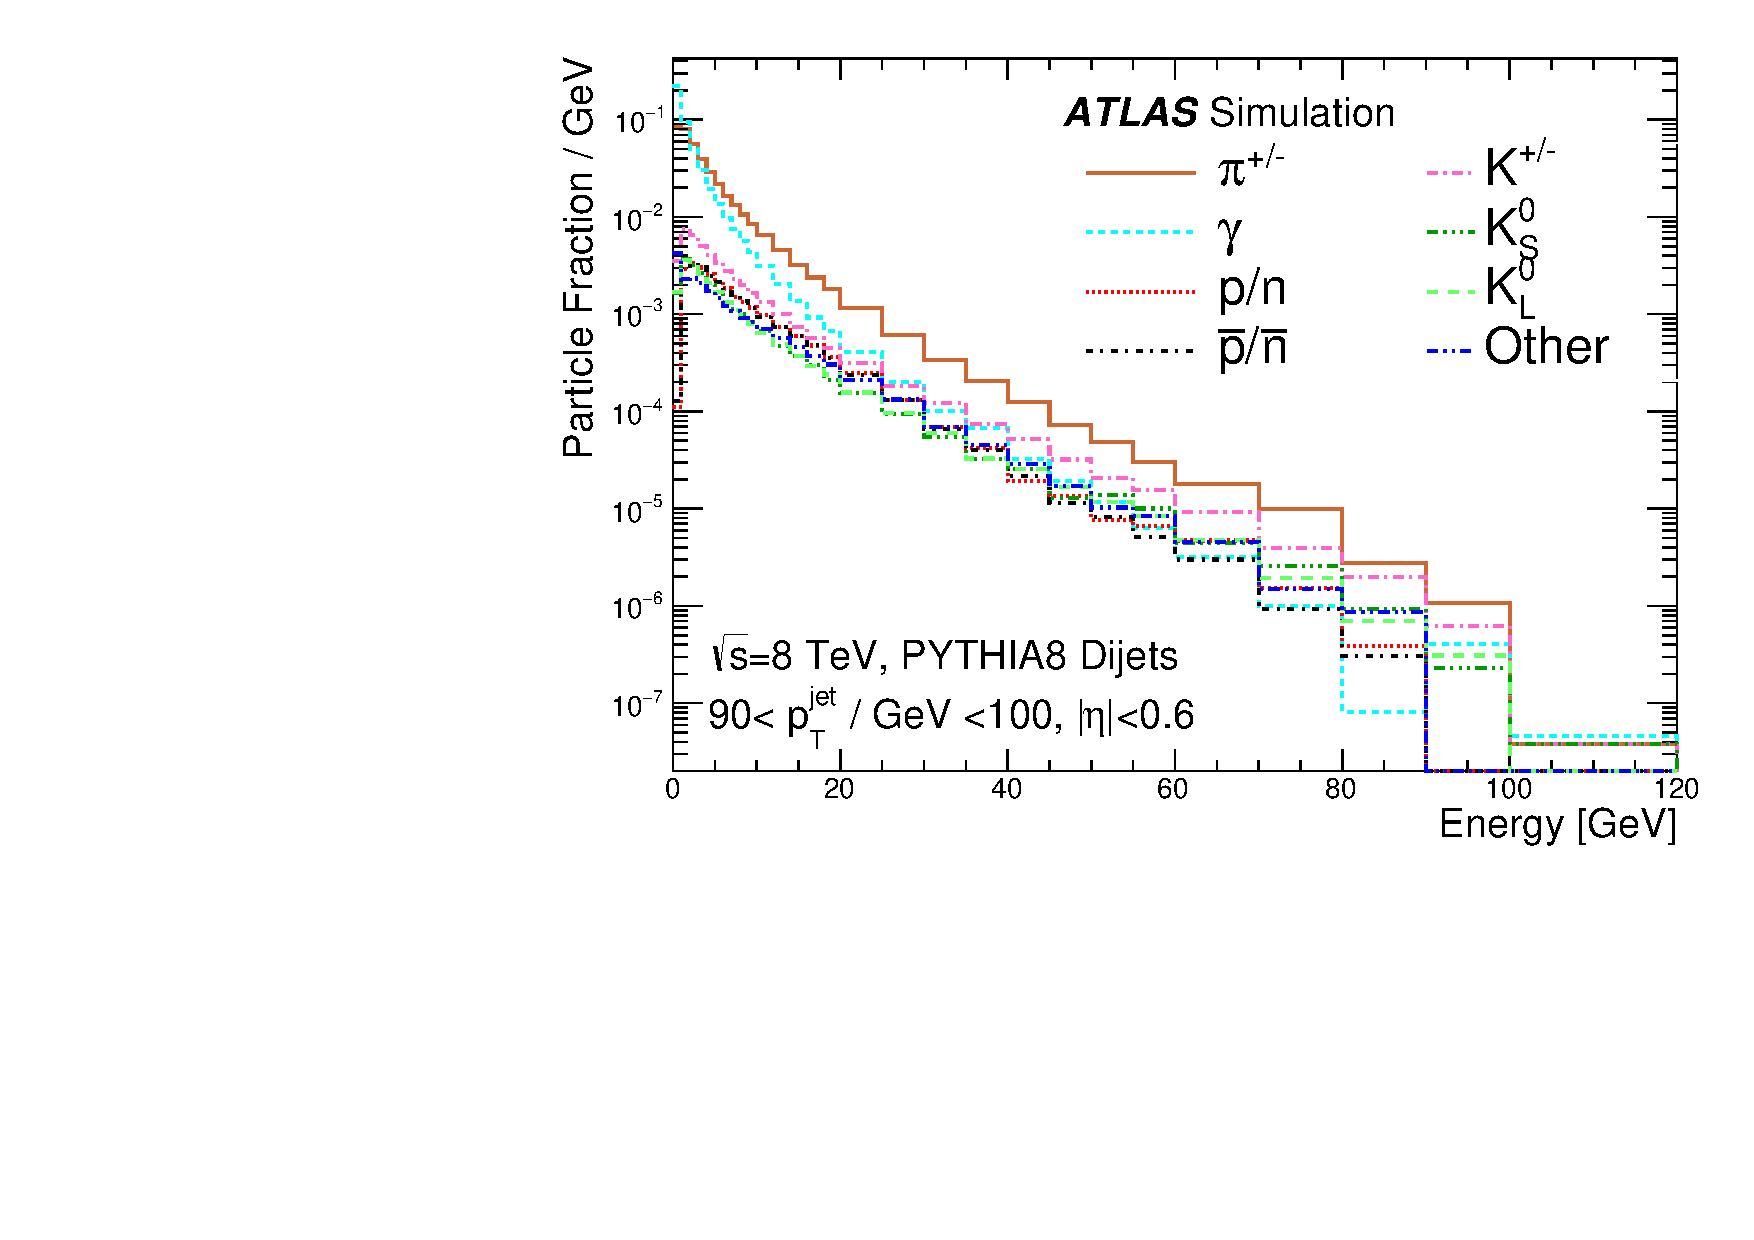
\includegraphics[width=0.48\textwidth]{figures/particle_spectra_90to100.pdf}
}
\subfloat[]{
  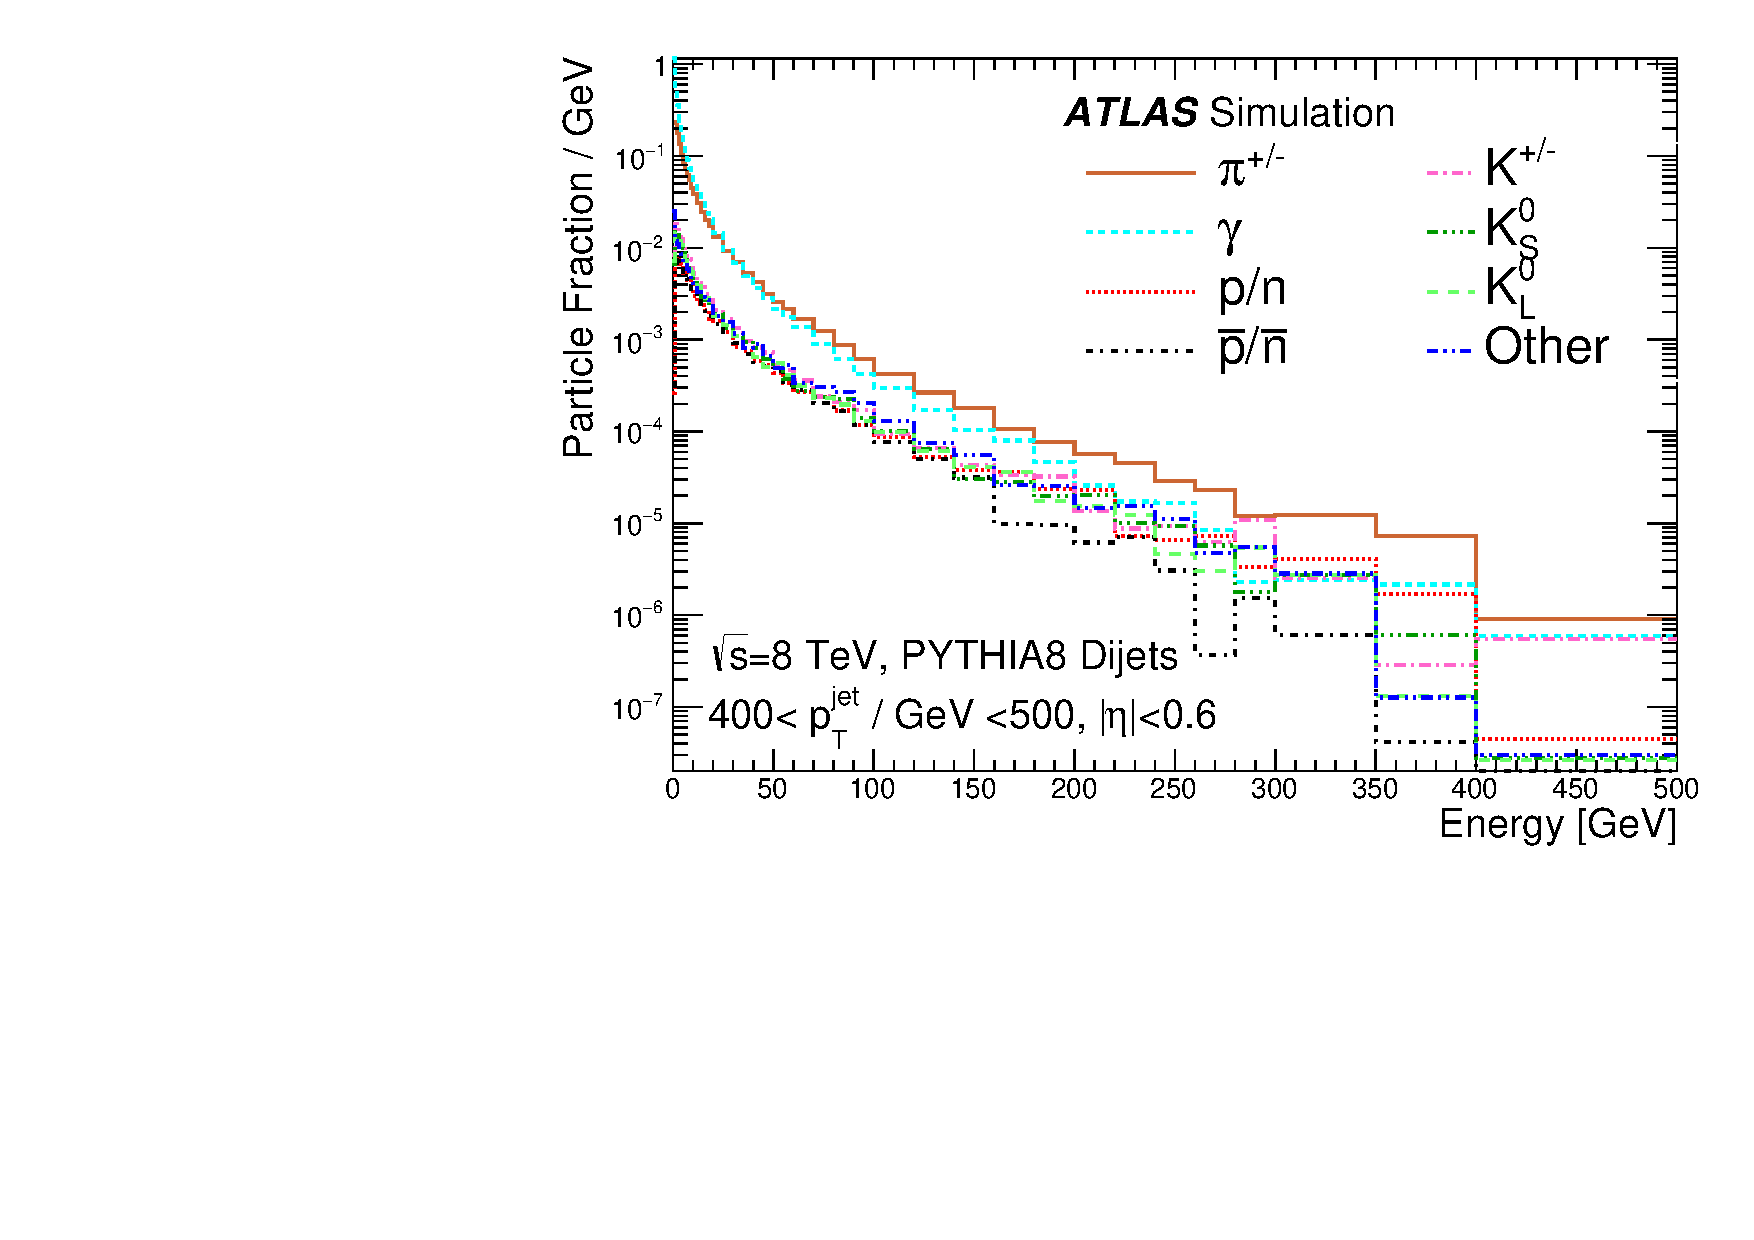
\includegraphics[width=0.48\textwidth]{figures/particle_spectra_400to500.pdf}
}\\
\subfloat[]{
  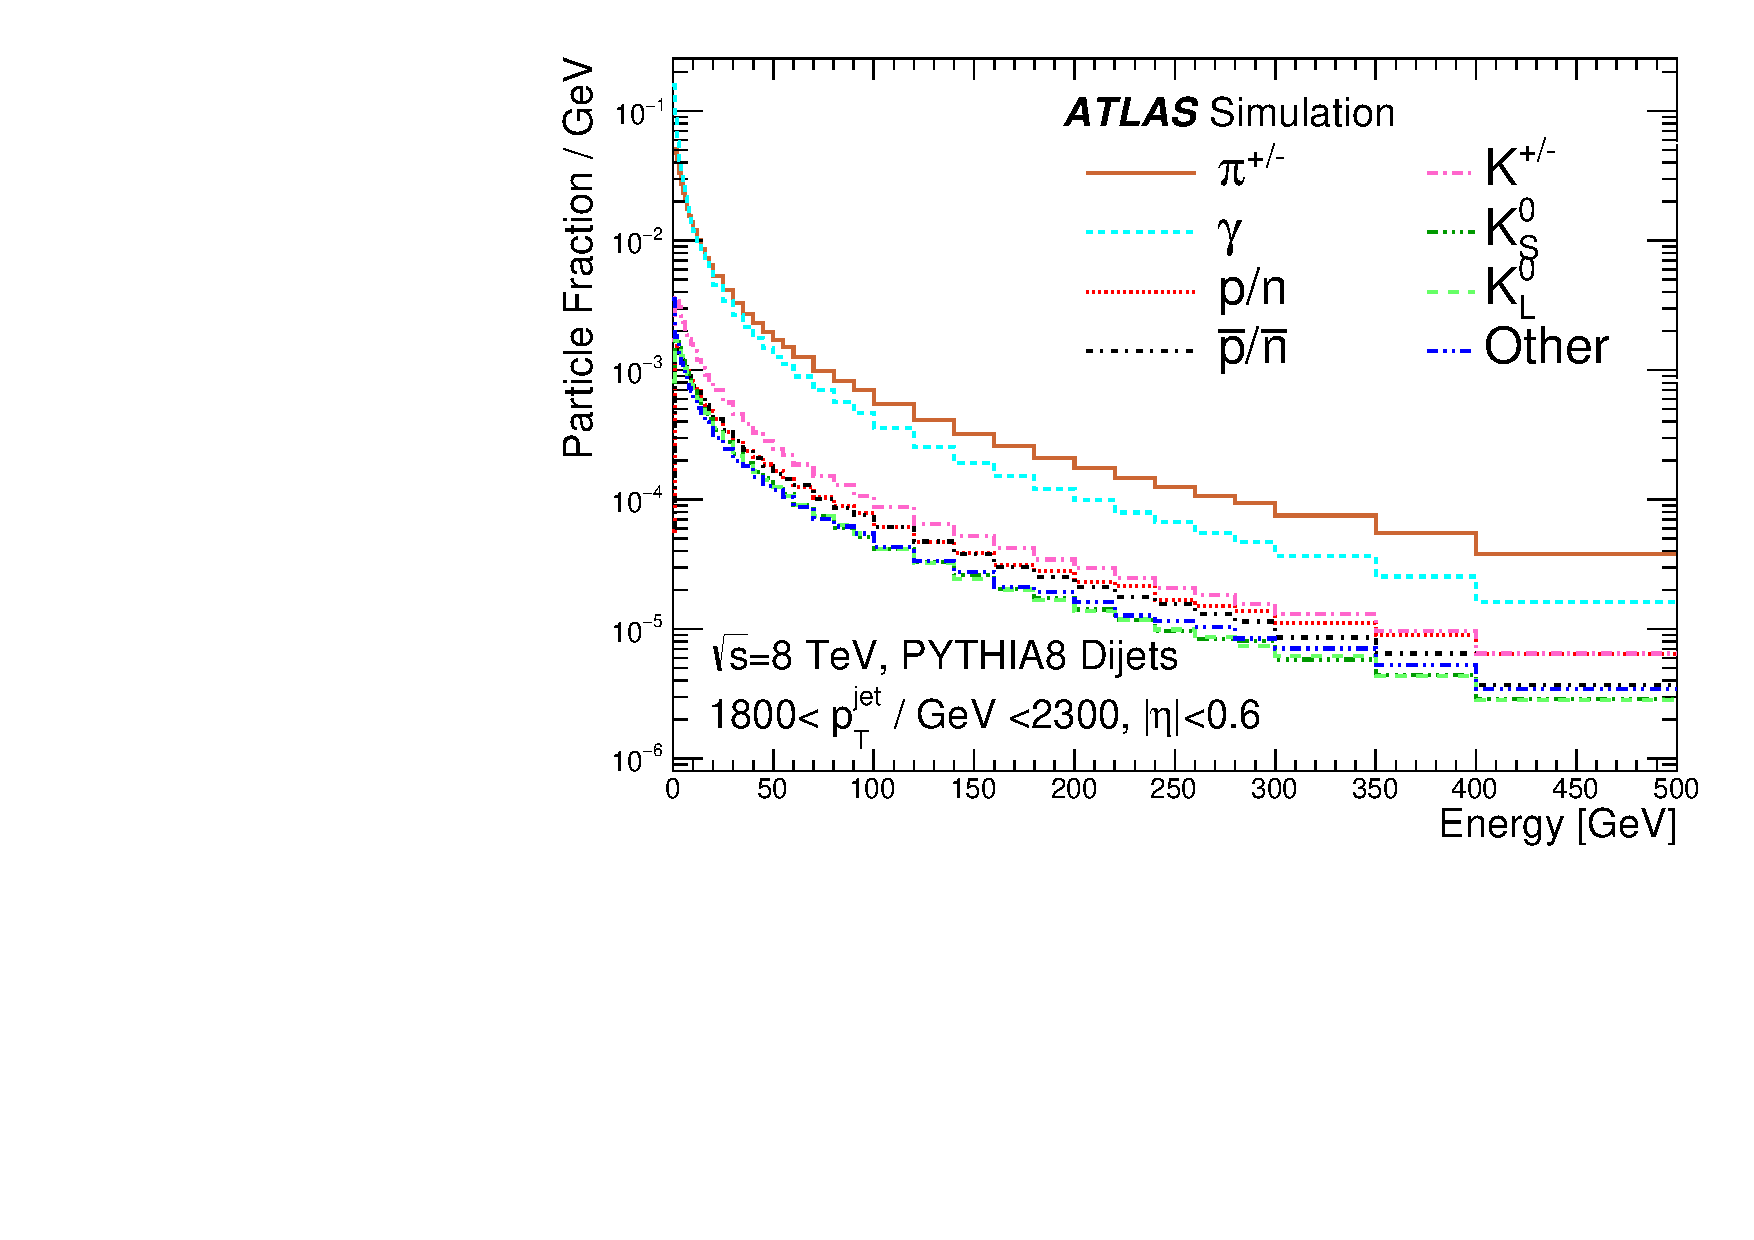
\includegraphics[width=0.48\textwidth]{figures/particle_spectra_1800to2300.pdf}
}
\caption{The spectra of true particles inside anti-$k_t$, $R=0.4$ jets with (a) $90<\pt/\GeV<100$, (b) $400<\pt/\GeV<500$, and (c) $1800<\pt/\GeV<2300$.}
\label{fig:particle_spectra}
\end{figure}

\section{Uncertainty Estimate}

Simulated jets are not necessarily expected to correctly model the energy deposits in the calorimeters, because of the various discrepancies discussed in Chapter~\ref{ch:singlehadrons}.
To evaluate a jet energy response, the simulated jet energies are compared to a corrected jet built up at the particle level.
Each cluster in a jet is associated to the truth particle which deposited it, and the energy in that cluster is then corrected for a number of effects based on measurements in data. 
The primary corrections come from the single hadron response measurements in addition to response measured using the combined test beam which covers higher momentum particles~\cite{CTB}.
These corrections include both a shift ($\Delta$), in order to make the simulation match the average response in data, and an uncertainty ($\sigma$) associated with the ability to constrain the difference between data and simulation.
Some of the dominant sources of uncertainty are itemized in Table~\ref{tab:jes_sources} with typical values, and the full list considered is described in detail in the associated paper~\cite{PERF-2015-05}. 
These uncertainties cover differences between the data and simulation in the modeling of calorimeter response to a given particle.
No uncertainties are added for the difference between particle composition of jets in data and simulation.


\begin{table}
\begin{tabular}{l p{.6\textwidth} c c}
\hline
Abbrev. & Description & $\Delta$ (\%) & $\sigma$ (\%)\\
\hline
In situ $E/p$ & The comparison of \epcor as described in Chapter~\ref{ch:singlehadrons} with statistical uncertainties from 500~\MeV\ to 20~\GeV. & 0-3 & 1-5 \\
CTB & The main \epav comparison uncertainties, binned in $p$ and $|\eta|$, as derived from the combined test beam results, from 20 to 350~\GeV~\cite{CTB}. & 0-3 & 1-5 \\
$E/p$ Zero Fraction & The difference in the zero-fraction between data and MC simulation from 500~\MeV\ to 20~\GeV. & 5-25 & 1-5 \\
$E/p$ Threshold & The uncertainty in the EM calorimeter response from the potential mismodeling of threshold effects in topological clustering. & 0 & 0-10 \\
Neutral & The uncertainty in the calorimeter response to neutral hadrons based on studies of physics model variations. & 0 & 5-10 \\
$K_\text{L}$ & An additional uncertainty in the response to neutral \pKL in the calorimeter based on studies of physics model variations. & 0 & 20 \\
$E/p$ Misalignment & The uncertainty in the $p$ measurement from misalignment of the ID. & 0 & 1 \\
Hadrons, $p>350$~\GeV & A flat uncertainty for all particles above the energy range or outside the longitudinal range probed with the combined test beam. & 0 & 10 \\
\hline
\end{tabular}
\label{tab:jes_sources}
\caption{The dominant sources of corrections and systematic uncertainties in the \ac{JES} estimation technique, including typical values for the correcting shift ($\Delta$) and the associated uncertainty ($\sigma$).}
\end{table}

From these terms, the \acl{JES} and uncertainty is built up from individual energy deposits in simulation. 
Each uncertainty term is treated independently, and are taken to be gaussian distributed.
The resulting scale and uncertainty is shown in Figure~\ref{fig:jes_uncertainty}, where the mean response is measured relative to the calibrated energy reported by simulation.
The dominant uncertainties come from the statistical uncertainties on the \ep measurements at lower energies and the additional uncertainty for out of range measurements at higher energies. 
The total uncertainty from this method at intermediate jet energies is comparable to other simulation-based methods~\cite{PERF-2011-03} and is about twice as large as in-situ methods using data~\cite{PERF-2012-01}. 
This method is the only one which provides an estimation above 1.8 \TeV, however, and so is still a crucial technique in analyses that search for very energetic jets.

\begin{figure}[ht]
\centering
\subfloat[]{
  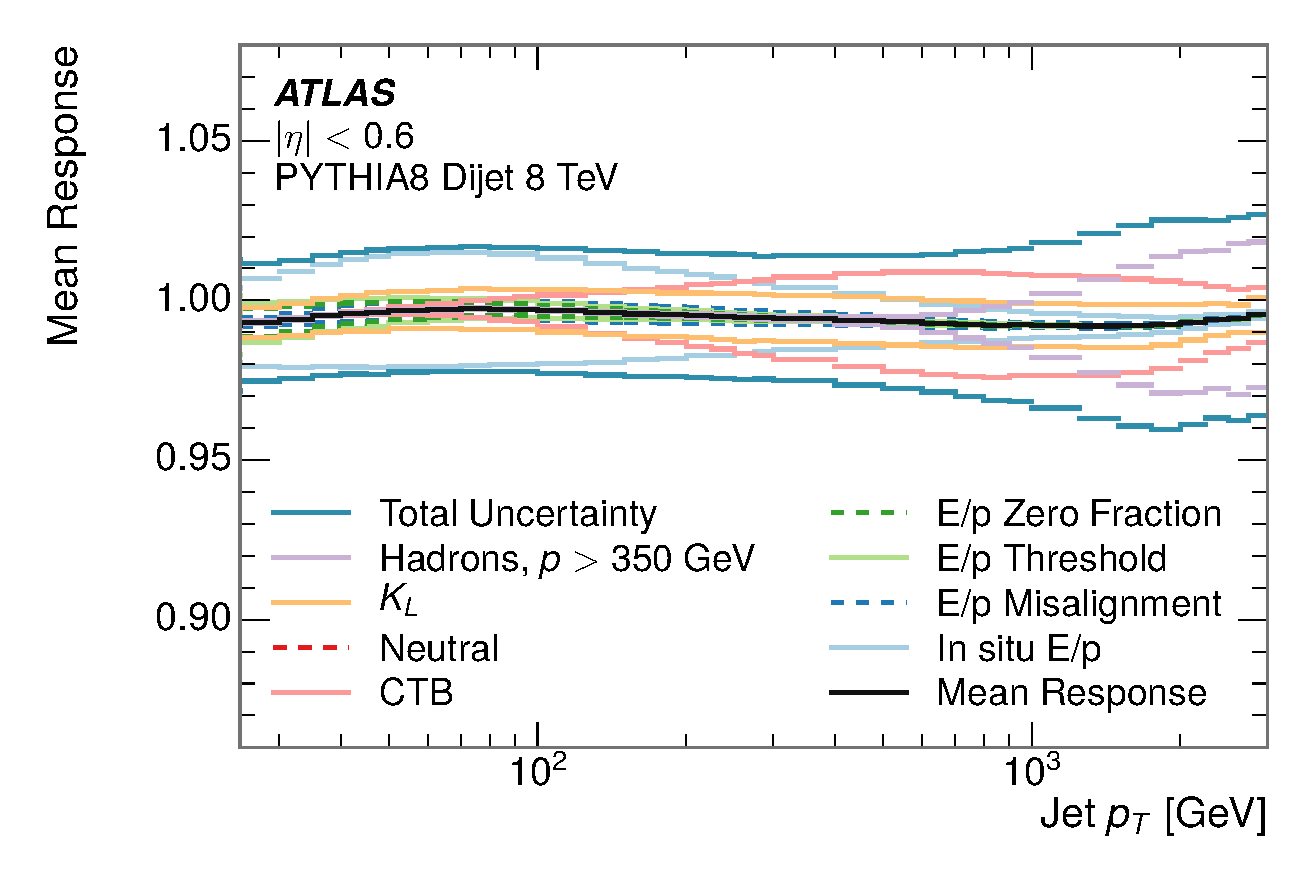
\includegraphics[width=0.85\textwidth]{figures/mc12jes_response_eta01.pdf}
} \\
\subfloat[]{
  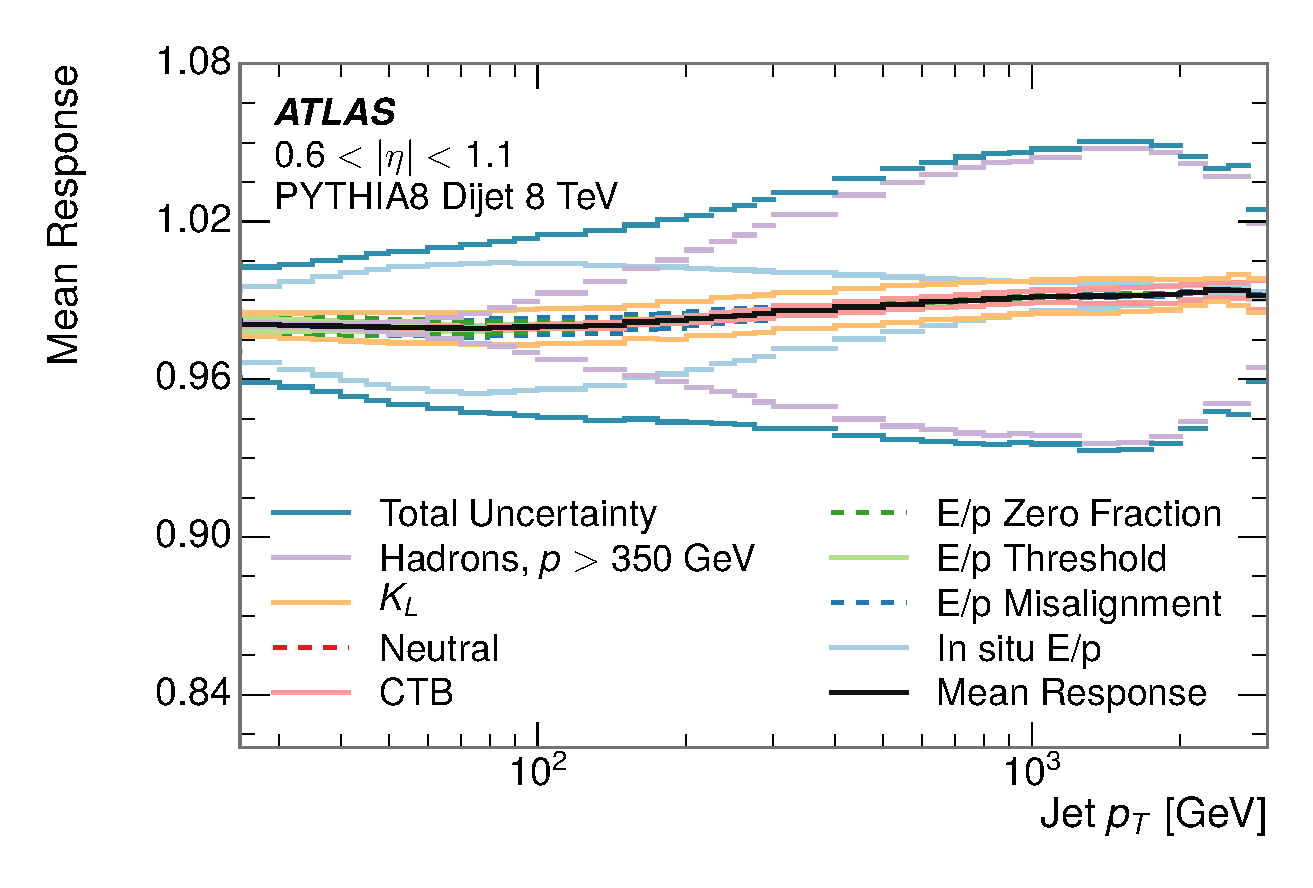
\includegraphics[width=0.85\textwidth]{figures/mc12jes_response_eta02.pdf}
}
\caption{ The \ac{JES} uncertainty contributions, as well as the total \ac{JES} uncertainty, as a function of jet $\pt$ for (a) $|\eta| < 0.6$ and (b) $0.6 < |\eta| < 1.1$.}
\label{fig:jes_uncertainty}
\end{figure}

These techniques can also be used to measure the correlation between bins of average reconstructed jet momentum across a range of $p_T$ and $|\eta|$, where correlations are expected because of a similarity in particle composition at similar energies.
Figure~\ref{fig:jes_correlations} shows these correlations, where the uncertainties on jets in neighboring bins are typically between 30\% and 60\% correlated. 
The uncertainty on all jets becomes significantly correlated at high energies and larger pseudorapidities, when the uncertainty becomes dominated by the single term reflecting out of range particles.

\begin{figure}[ht]
\centering
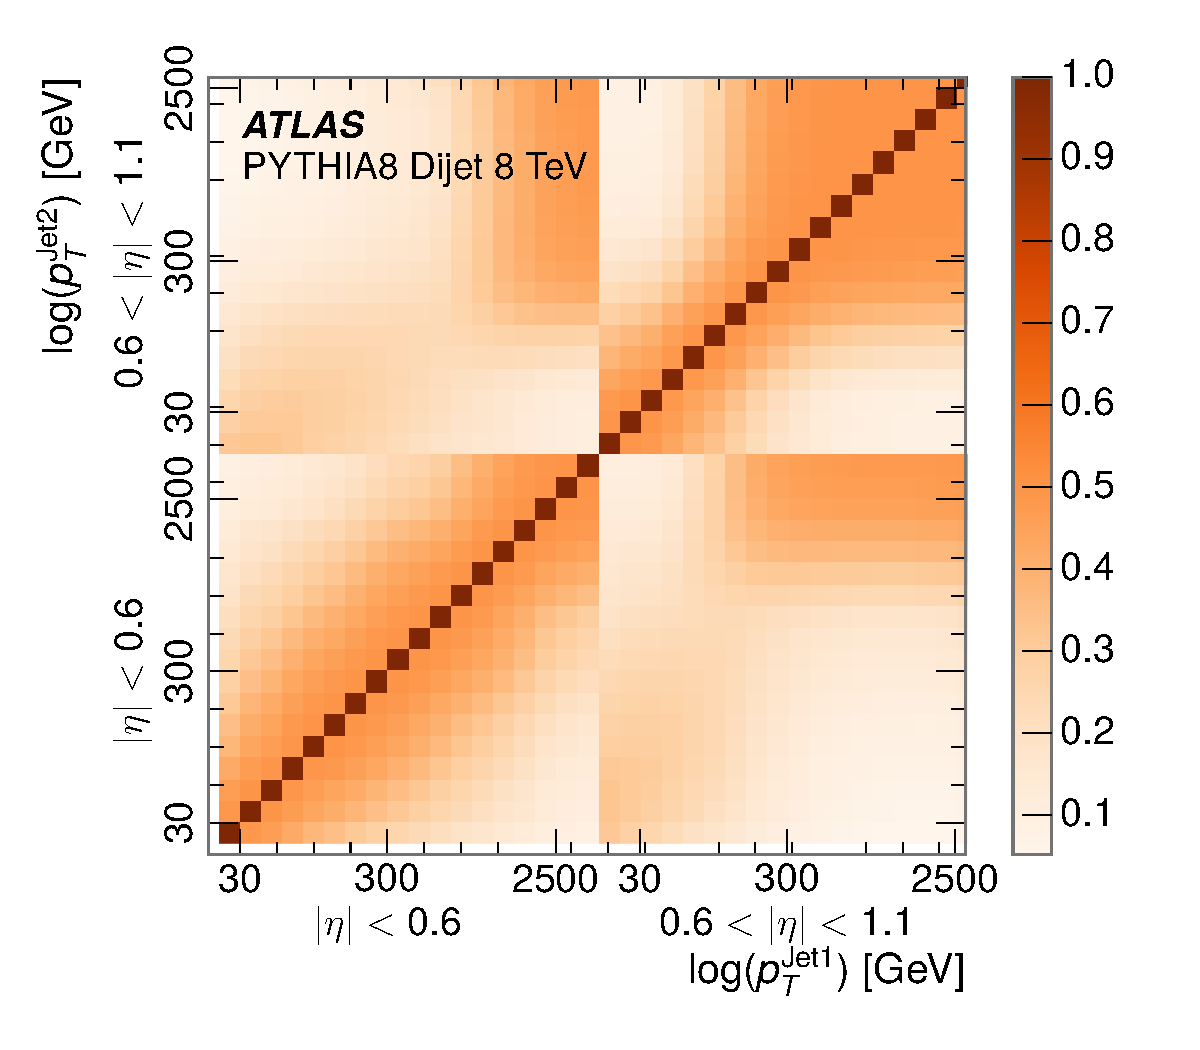
\includegraphics[width=0.7\textwidth]{figures/correlation.pdf}
\caption{ The \ac{JES} correlations as a function of jet $\pt$ and $|\eta|$ for jets in the central region of the detector.}
\label{fig:jes_correlations}
\end{figure}

\section{Summary}
The technique described above provides a \acl{JES} and uncertainty by building up jet corrections from the energy deposits of constituent particles.
The \ep measurements are crucial in providing corrections for the majority of particles in the jets.
The uncertainty derived this way is between 2 and 5\% and is about twice as large at corresponding momentum than jet balance methods.
However this is the only uncertainty available for very energetic jets using 2012 data and simulation, and repeating this method with Run 2 data and simulation will be important in providing an uncertainty for the most energetic jets in 13 \TeV collisions.

% ----------------------------------------
